%%%%%%%%%%%%%%%%%%%%%%%%%%%%%%%%%%%%%%%%%
% Wenneker Assignment
% LaTeX Template
% Version 2.0 (12/1/2019)
%
% This template originates from:
% http://www.LaTeXTemplates.com
%
% Authors:
% Vel (vel@LaTeXTemplates.com)
% Frits Wenneker
%
% License:
% CC BY-NC-SA 3.0 (http://creativecommons.org/licenses/by-nc-sa/3.0/)
% 
%%%%%%%%%%%%%%%%%%%%%%%%%%%%%%%%%%%%%%%%%

%----------------------------------------------------------------------------------------
%	PACKAGES AND OTHER DOCUMENT CONFIGURATIONS
%----------------------------------------------------------------------------------------

\documentclass[11pt]{scrartcl} % Font size

%%%%%%%%%%%%%%%%%%%%%%%%%%%%%%%%%%%%%%%%%
% Wenneker Assignment
% Structure Specification File
% Version 2.0 (12/1/2019)
%
% This template originates from:
% http://www.LaTeXTemplates.com
%
% Authors:
% Vel (vel@LaTeXTemplates.com)
% Frits Wenneker
%
% License:
% CC BY-NC-SA 3.0 (http://creativecommons.org/licenses/by-nc-sa/3.0/)
% 
%%%%%%%%%%%%%%%%%%%%%%%%%%%%%%%%%%%%%%%%%

%----------------------------------------------------------------------------------------
%	PACKAGES AND OTHER DOCUMENT CONFIGURATIONS
%----------------------------------------------------------------------------------------

\usepackage{amsmath, amsfonts, amsthm} % Math packages

\usepackage{listings} % Code listings, with syntax highlighting
\usepackage[outputdir=out]{minted}

\usepackage[english]{babel} % English language hyphenation

\usepackage{graphicx} % Required for inserting images
\graphicspath{{Figures/}{./}} % Specifies where to look for included images (trailing slash required)

\usepackage{booktabs} % Required for better horizontal rules in tables

\numberwithin{equation}{section} % Number equations within sections (i.e. 1.1, 1.2, 2.1, 2.2 instead of 1, 2, 3, 4)
\numberwithin{figure}{section} % Number figures within sections (i.e. 1.1, 1.2, 2.1, 2.2 instead of 1, 2, 3, 4)
\numberwithin{table}{section} % Number tables within sections (i.e. 1.1, 1.2, 2.1, 2.2 instead of 1, 2, 3, 4)

\setlength\parindent{0pt} % Removes all indentation from paragraphs

\usepackage{enumitem} % Required for list customisation
\setlist{noitemsep} % No spacing between list items

%----------------------------------------------------------------------------------------
%	DOCUMENT MARGINS
%----------------------------------------------------------------------------------------

\usepackage{geometry} % Required for adjusting page dimensions and margins

\geometry{
	paper=a4paper, % Paper size, change to letterpaper for US letter size
	top=2.5cm, % Top margin
	bottom=3cm, % Bottom margin
	left=3cm, % Left margin
	right=3cm, % Right margin
	headheight=0.75cm, % Header height
	footskip=1.5cm, % Space from the bottom margin to the baseline of the footer
	headsep=0.75cm, % Space from the top margin to the baseline of the header
	%showframe, % Uncomment to show how the type block is set on the page
}

%----------------------------------------------------------------------------------------
%	FONTS
%----------------------------------------------------------------------------------------

\usepackage[utf8]{inputenc} % Required for inputting international characters
\usepackage[T1]{fontenc} % Use 8-bit encoding

\usepackage{fourier} % Use the Adobe Utopia font for the document

%----------------------------------------------------------------------------------------
%	SECTION TITLES
%----------------------------------------------------------------------------------------

\usepackage{sectsty} % Allows customising section commands

\sectionfont{\vspace{6pt}\centering\normalfont\scshape} % \section{} styling
\subsectionfont{\normalfont\bfseries} % \subsection{} styling
\subsubsectionfont{\normalfont\itshape} % \subsubsection{} styling
\paragraphfont{\normalfont\scshape} % \paragraph{} styling

%----------------------------------------------------------------------------------------
%	HEADERS AND FOOTERS
%----------------------------------------------------------------------------------------

\usepackage{scrlayer-scrpage} % Required for customising headers and footers

\ohead*{} % Right header
\ihead*{} % Left header
\chead*{} % Centre header

\ofoot*{} % Right footer
\ifoot*{} % Left footer
\cfoot*{\pagemark} % Centre footer
 % Include the file specifying the document structure and custom commands

%----------------------------------------------------------------------------------------
%	TITLE SECTION
%----------------------------------------------------------------------------------------

\title{	
	\normalfont\normalsize
	\begin{center}
		\begin{minipage}[c]{0.2\textwidth}
			\textsc{\Large SZ-Ybbs}
		\end{minipage}%
		\begin{minipage}[c]{0.1\textwidth}
			
\includegraphics[width=\textwidth]{LogoITHTL_white.pdf}
		\end{minipage}
	\end{center}
	\vspace{10pt} % Whitespace
	\rule{\linewidth}{0.5pt}\\ % Thin top horizontal rule
	\vspace{20pt} % Whitespace
	{\huge 4G}\\ % The assignment title
	\vspace{12pt} % Whitespace
	\rule{\linewidth}{2pt}\\ % Thick bottom horizontal rule
	\vspace{12pt} % Whitespace
}

\author{\LARGE Erber Jakob \and \LARGE Freunberger Raphael} % Your name

\date{\normalsize\today} % Today's date (\today) or a custom date

\begin{document}

\maketitle % Print the title

\tableofcontents
\clearpage

\section{Introduction}
This paper explores key technologies that enable the efficient operation of 4G wireless networks, with a particular focus on Orthogonal Frequency Division Multiple Access (OFDMA) and Multiple-Input Multiple-Output (MIMO) systems. The first part of the paper examines the fundamental requirements of a 4G network, followed by an in-depth analysis of OFDMA, a key multiple access technique used in modern communication systems. OFDMA's advantages over traditional frequency division multiplexing (FDM) and its ability to efficiently allocate subcarriers among multiple users are highlighted. The paper then delves into MIMO technology, which utilizes multiple antennas to improve data rates and reliability, and its various configurations and applications within 4G networks. Together, OFDMA and MIMO represent the backbone of 4G wireless communication, enabling high-speed, robust, and scalable mobile connectivity.

\section{Requirements of a 4G Network}
Since Proxmox focuses on smaller environments with weaker hardware the hardware requirements to run Proxmox are very low. Pretty much any AMD or Intel system manufactured within the last 10 years should meet the requirements.

\begin{itemize}
	\item x86-64 CPU with VT/AMD-V enabled
	\item 2GB memory
	\item About 16GB disk space for the hypervisors OS
\end{itemize}

\subsection{vSphere}
For vSphere the requirements are higher and only Intel Xeon, AMD Epyc and some specific SKUs of the intel core series are officially supported. 
If you try to install ESXi v8 on an unsupported CPU you will get a warning and can only choose to reboot the system. There is a workaround with a kernel flag, but you will almost certainly not get any support from VMWare if you do so. 

\begin{itemize}
	\item x86-64 CPU with at least 2 cores with VT/AMD-V enabled
	\item 8GB memory
	\item 32GB boot disk
\end{itemize}

\section{OFDMA - Erber Jakob}
Orthogonal frequency-division multiplexing (OFDM) and the multi user variant OFDMA are in nearly all modern wireless communication systems, including 4G, 5G, and Wi-Fi 6. OFDM is a modulation technique that divides the available spectrum into multiple orthogonal subcarriers. This allows for high spectral efficiency and robustness against frequency-selective fading. OFDMA is a multiple access scheme that allows multiple users to share the same frequency band by assigning different subcarriers to different users.

\subsection{FDM}

But lets start with Frequency Division Multiplexing (FDM) first, which is used in FM radio. In FDM the available frequency band is divided into multiple non-overlapping subbands, each of which is used by a different user. Between the subbands are guard bands to prevent interference between the users. This is a very inefficient use of the spectrum.

\begin{figure}[H]
	\centering
	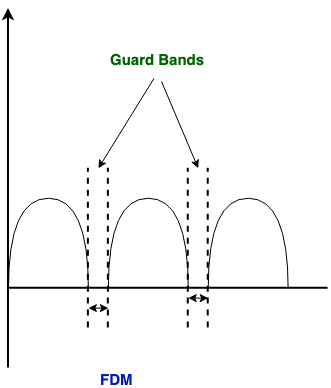
\includegraphics[width=0.3\textwidth]{Figures/fdm.png}
	\caption{Frequency Division Multiplexing}
\end{figure}

\subsection{OFDM}

OFDM is a more efficient way to divide the spectrum. Instead of using non-overlapping subbands, OFDM divides the spectrum into multiple orthogonal subcarriers. This means that the subcarriers can be spaced closer together, allowing for a higher spectral efficiency. The orthogonality of the subcarriers means that they do not interfere with each other, even when they are spaced closely together. The peaks of the subcarriers line up with the nulls of the other subcarriers, as can be seen in the figure below.

\begin{figure}[H]
	\centering
	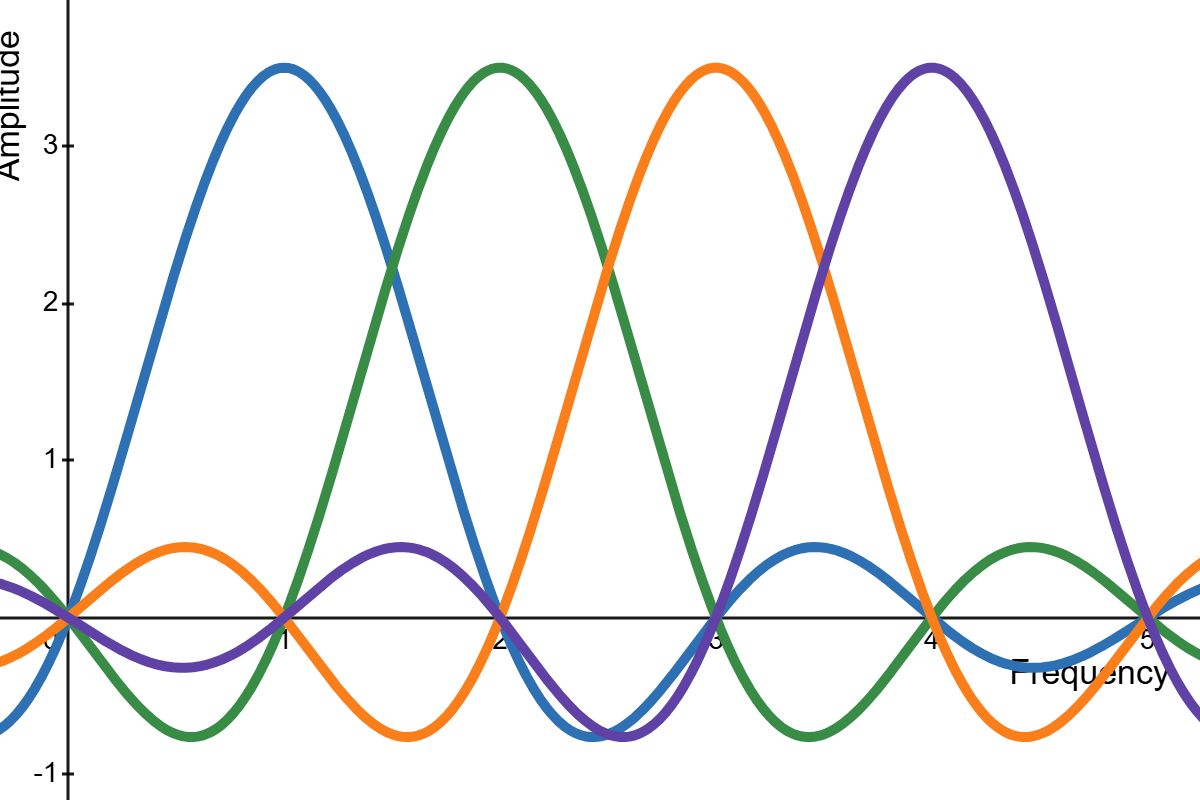
\includegraphics[width=0.4\textwidth]{Figures/ofdm.png}
	\caption{Orthogonal Frequency Division Multiplexing}
\end{figure}

\subsection{OFDMA}

In OFDMA users are dynamically assigned a subset of the subcarriers, depending on their data rate requirements. This reallocation happens very fast, on the order of single milli seconds. Bad subnets, for example due to high frequency fading, are not assigned to users. This allows for a more efficient use of the spectrum and better performance in the presence of fading.

Compared to the other multiple access schemes, FDMA, TDMA, and CDMA, OFDMA has several advantages. It is more robust against frequency-selective fading, it allows for a more efficient use of the spectrum, and it is more flexible in terms of the number of users that can be supported. Ther higher complexity of OFDMA is a price most wireless technologies are willing to pay for the advantages it offers.

\section{MIMO - Freunberger Raphael}
\textbf{MIMO} (or \textbf{m}ultiple-\textbf{i}nput and \textbf{m}ultiple-\textbf{o}utput) is a technology that uses multiple antennas to increase the capacity of a wireless link. 
It is a key technology in modern wireless communication systems, including 4G networks and Wi-Fi. 
MIMO technology takes advantage of \textbf{multi-path propagation}, which means that signals can take multiple paths between the transmitter and receiver caused by reflections, diffractions, and scattering. 
By using multiple antennas at both the transmitter and receiver, MIMO technology can exploit these multiple paths to increase the data rate and reliability of the wireless link.

\begin{figure}[H]
	\centering
	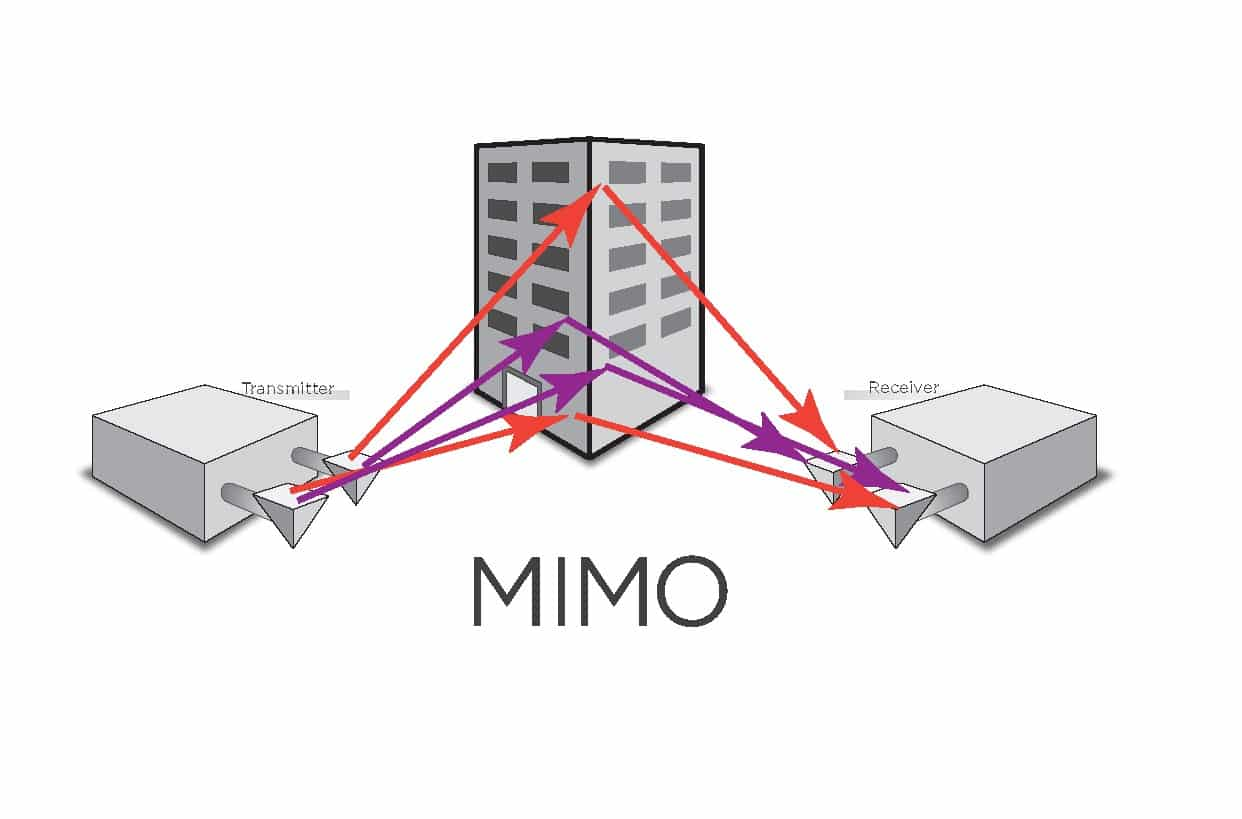
\includegraphics[width=0.4\textwidth]{Figures/mimo.png}
	\caption{Multiple-Input Multiple-Output (MIMO) system} 
\end{figure}

A early predecessor of MIMO technology is \textbf{Space-division multiple access} (SDMA), which used directional antennas to reach multiple users in different directions on the same frequency-band. MIMO technology, on the other hand, uses multiple antennas to transmit multiple data streams on the same frequency-band to the same user.


\subsection{Functions of MIMO}

\paragraph{Channel State Information (CSI)}
Channel State Information (CSI) refers to the knowledge of the communication channel’s characteristics, including attenuation, delay, and fading. 
It helps optimize transmission by adjusting power, phase, and modulation. 
CSI is estimated at the receiver and sent back to the transmitter. 
Accurate CSI is essential for techniques like beamforming and precoding to enhance signal strength and reduce interference.


\paragraph{Precoding and Beamforming}
Precoding is multi-stream beamforming that occurs at the transmitter. 
Beamforming adjusts phase and gain to maximize signal power at the receiver. 
It increases signal strength and reduces multipath fading. 
Precoding with multiple streams is useful when the receiver has multiple antennas and requires CSI.

\paragraph{Spatial Multiplexing}
Spatial multiplexing splits a high-rate signal into lower-rate streams, each transmitted from a different antenna. 
The receiver can separate the streams if it has accurate CSI. 
This technique increases capacity, especially at high SNR. 
The number of streams is limited by the smaller antenna count. 
It can work without CSI at the transmitter and can also support multi-user MIMO with CSI.

\paragraph{Diversity Coding}
Diversity coding transmits a single stream with space-time coding for reliability. 
It exploits independent fading across antennas but does not provide beamforming gains. 
When some CSI is available, diversity coding can combine with spatial multiplexing to improve performance.


\subsection{Variations of MIMO}

Different variations of MIMO systems include:

\begin{itemize}
    \item \textbf{Single-User MIMO (SU-MIMO):} 
    A MIMO system where multiple antennas are used at both the transmitter and receiver to improve data rates and reliability for a single user, using spatial multiplexing to transmit multiple data streams simultaneously.
    
    \item \textbf{Multi-User MIMO (MU-MIMO):} 
    Allows a base station to communicate with multiple users simultaneously, each with multiple antennas. This technique increases system capacity by enabling space-division multiple access (SDMA) based on spatial signatures of the users.
    
    \item \textbf{Massive MIMO:} 
    Involves a large number of antennas at the base station to serve many users simultaneously, greatly enhancing spectral and energy efficiency by exploiting spatial diversity.
    
    \item \textbf{Distributed MIMO:} 
    Utilizes multiple geographically separated antennas connected by a backhaul network, improving coverage and reliability over large areas by exploiting spatial diversity.
    
    \item \textbf{Cooperative MIMO:} 
    Involves collaboration between multiple devices (such as users or base stations) to transmit and receive signals, forming a virtual antenna array. This improves system performance through coordinated resource sharing.
\end{itemize}

\subsection{Antenna Configurations}

The amount of antennas used in a MIMO system on transmitter and receiver is referred to as the antenna configuration. 
Common configurations include 2x2, 4x4, 8x8, etc., where the first number represents the number of antennas on the transmitter and the second number represents the number of antennas on the receiver.
\begin{figure}[H]
	\centering
	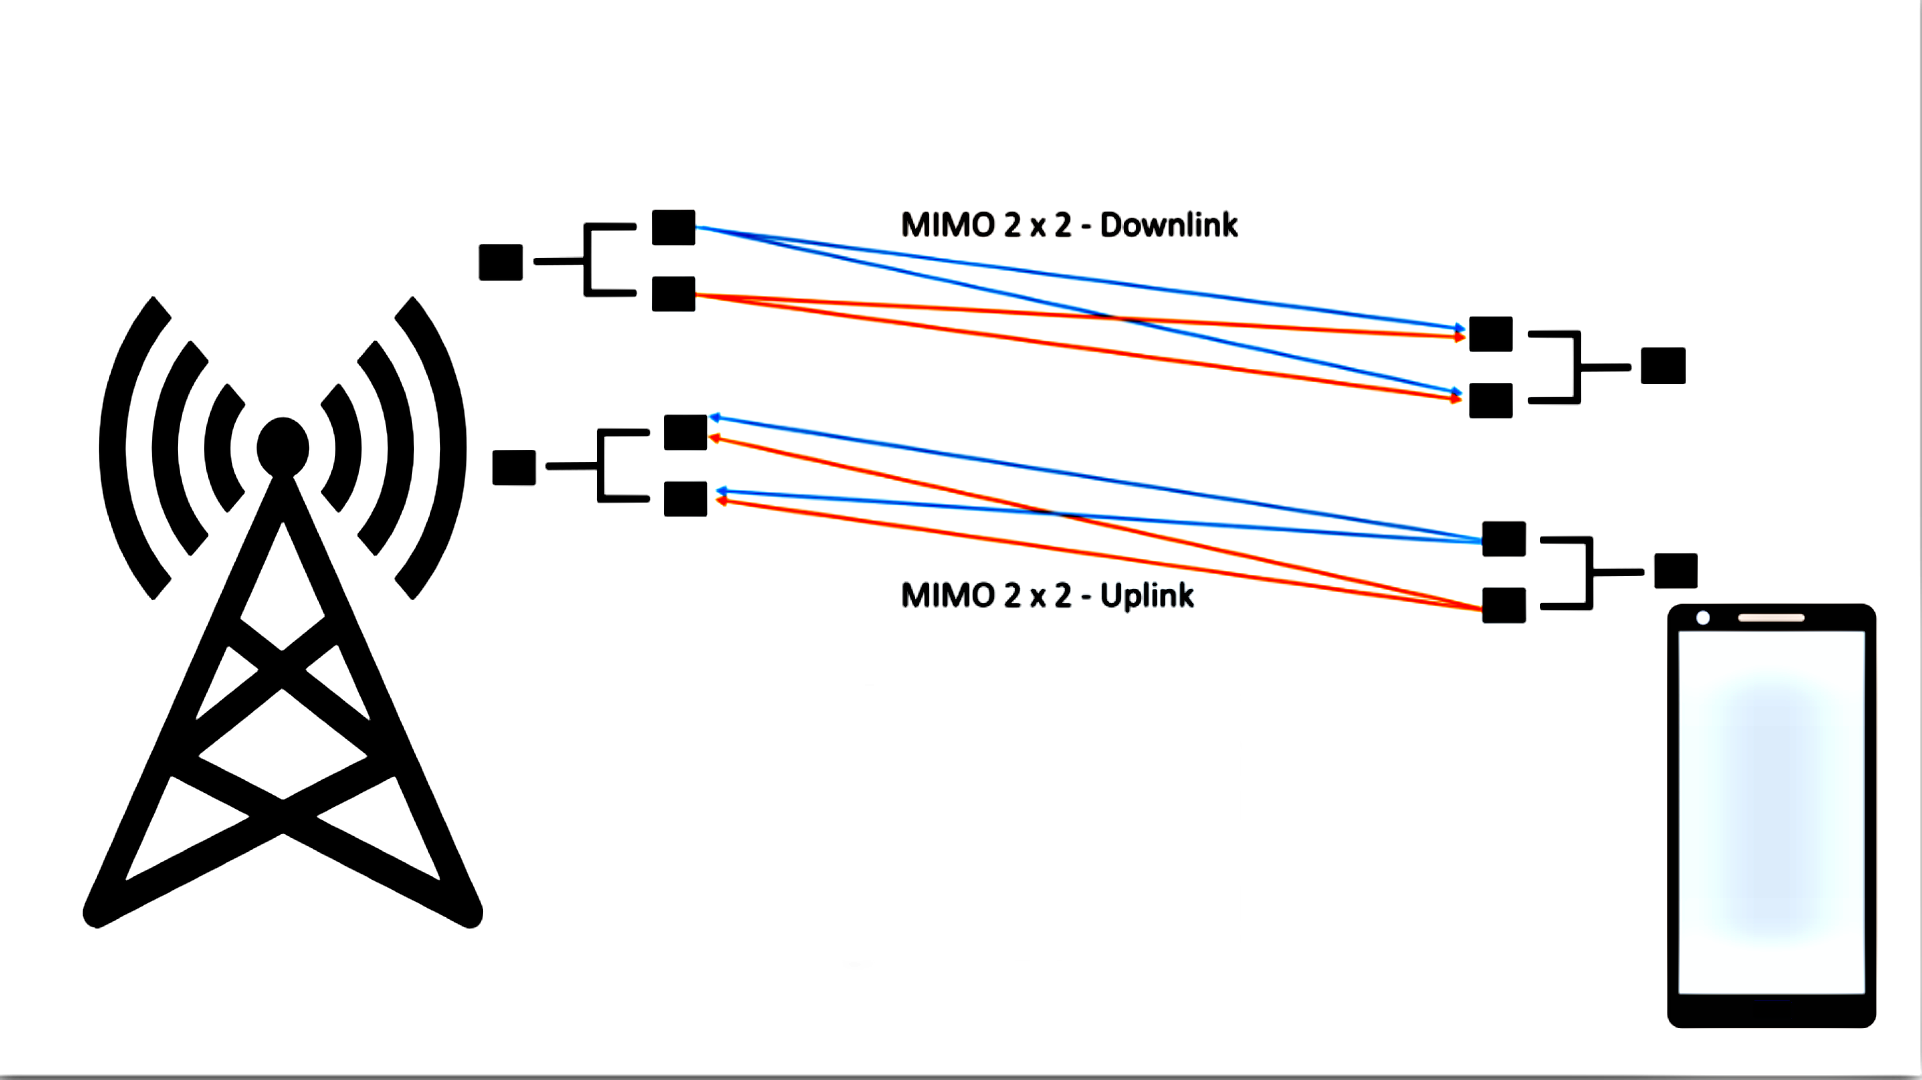
\includegraphics[width=0.6\textwidth]{Figures/mimo2x2.png}
	\caption{MIMO 2x2 Uplink and Downlink} 
\end{figure}

\subsubsection{MIMO in 4G Networks}

The 3rd Generation Partnership Project (3GPP) has defined different MIMO configurations for LTE, LTE Advanced, and LTE Advanced Pro networks.

\begin{table}[H]
    \centering
    \begin{tabular}{|l|l|l|}
    \hline
    \textbf{LTE Technology}      & \textbf{3GPP Release} & \textbf{Antenna Configuration (MIMO)} \\ \hline
    LTE                          & Release 8             & 4 x 4 Downlink \newline 2 x 2 Uplink  \\ \hline
    LTE Advanced                 & Release 10            & 8 x 8 Downlink \newline 4 x 4 Uplink  \\ \hline
    LTE Advanced Pro             & Release 13            & 8 x 8 Downlink \newline 4 x 4 Uplink  \\ \hline
    \end{tabular}
    \caption{MIMO configurations in LTE networks}
\end{table}
    

\end{document}